\documentclass[../../thesis.tex]{subfiles}

\begin{document}
This thesis covers a lot of ground and the field of machine learning draws on many parts of mathematics, statistics and computational sciences. As much as the author would love deep diving into every aspect, certain sections are somewhat superficial. There are though, for the interested reader, a large number of sources going into greater detail referenced throughout. \newline

In this section we begin by introducing neural networks, and relevant architectures for our work, such as convolutional neural networks and transformers. We give an intruduction to representation learning, highlighting standard evaluation protocols, and give an introduction to self-supervised learning (SSL), with emphasis on siamese architecture-based SSL. We present the Vector Quantized Variational Autoencoder, trying to highlight aspects brushed over in \cite{VQVAE}, building it up from Autoencoders. Before finally we go through the evaluation metrics used to assess our models.

% \section{Notation}

% \begin{itemize}
%     \item Encoder $E$
%     \item Decoder $D$
%     \item Estimated values are presented with a hat, $\widehat{x}$ for a reconstructed value, $\widehat{f}$ for a trained model etc.
%     \item Parameters $\theta$ 
%     \item Dataset $X = \{x_i\}_{i=1}^N$  
% \end{itemize}

% \section{Information theoretic/basic stats used in evaluation}

% - maximum entropy distribution

% - mutual information


% \begin{definition}[Differential entropy]
%     The differential entropy of a random variable $X$  with pdf or pmf $p$ defined on a sample space $\mathcal{X}$ is
%     \begin{equation}
%         h(X) =\E[-\log(f(X))] -\sum_{x\in \mathcal{X}} p(x)\log(p(x)),\text{ if $X$ is discrete,}
%     \end{equation}
%     \begin{equation}
%         h(X) =\E[-\log(f(X))] -\int_{\mathcal{X}} p(x)\log(p(x)),\text{ if $X$ is continuous}
%     \end{equation}
% \end{definition}


% - perplexity

% \begin{definition}[KL-Divergence]
%     For probability distribution $P$ and $Q$ defined on the same sample space $\mathcal{X}$, if for all $x\in\mathcal{X} $ $Q(x)=0$ implies $P(x)=0$, the Kullback-Leibler divergence is defined as
%     \begin{equation}
%         \KL(P||Q) = \sum_{x\in\mathcal{X}} P(x)\log\left(\frac{P(x)}{Q(x)}\right), \text{ if $P$ and $Q$ are discrete,}
%     \end{equation}
%     \begin{equation}
%         \KL(P||Q) = \int_{x} p(x)\log\left(\frac{p(x)}{q(x)}\right)dx, \text{ if $P$ and $Q$ are continuous}.
%     \end{equation}
% \end{definition}

% \url{https://stats.stackexchange.com/questions/188903/intuition-on-the-kullback-leibler-kl-divergence/189758#189758}

% - Cross entropy 

% - Graphical probabilistic models 
%     - Ancestral sampling

% - Generative models



\section{Neural Network}
An \textit{artificial neural network} or simply \textit{neural network} is a fundamental model in machine learning, and more specifically in \textit{deep learning}. Neural networks are loosely inspired by the way neurons are assembled in the brain. The concept dates back to 1943 when Warren McCulloch and Walter Pitts developed the first artificial neuron, which is considered the first neural model ever invented\cite{MCCULLOCH199099}. The first practical implementation was by Frank Rosenblatt in 1957 \cite{rosenblatt1957perceptron}. However, it wasn't until the development of the backpropagation algorithm in its modern form in the 1980s that neural networks gained significant traction. Since then, neural networks have been highly influential in the machine learning field, with a broad range of impressive applications, including face recognition, defeating humans in chess, Go, and Starcraft, self-driving cars, and predicting protein structures.
The remarkable effectiveness of neural networks across diverse tasks can partly be explained by the \textit{universal approximation theorem}, proven by Kurt Hornlik in 1989 \cite{HORNIK1989359}, which roughly states that a neural network can approximate any (Borel measurable) function to any desired degree of accuracy. \newline

\begin{figure}
    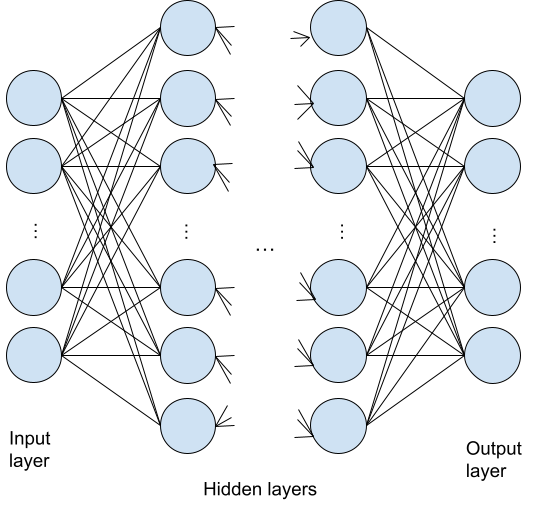
\includegraphics[scale = 0.4]{NeuralNet.png}
    \centering 
    \caption{Illustration of a Neural Network model.}
    \label{fig:NeuralNet}
\end{figure}

A neural network takes in a vector $x \in \mathbb{R}^n$ and builds a nonlinear function $f(x)$ to predict the response $y\in \mathbb{R}^m$. More specifically, a neural network maps an input vector $x$ to an output vector $y$ through a series of nonlinear functions applied to linear combinations of the input. This particular structure, illustrated in Figure \ref{fig:NeuralNet}, distinguishes neural networks from other nonlinear prediction models. \newline

The variables $x = [x_1,...,x_n]$ constitute the units of the \textit{input layer}. The intermediate layers are called the \textit{hidden layers}, and the final mapping to $y$ is called the \textit{output layer}. A neural network is parameterized by a set of \textit{weight} matrices $W_i$ and \textit{bias} vectors $b_i$, together with a specified set of non-linear \textit{activation functions} $\{\sigma_1,\dots,\sigma_{K-1}\}$. We denote the collection of parameters $\{W_1,...,W_{K-1}, b_1,...,b_{K-1}\}$ by $\theta$. Written out a $K$ layered neural network is given by 
\[ 
f_\theta(x) = f_K \circ f_{K-1} \circ \ldots \circ f_2 \circ f_1(x),
\]
where 
$$f_i(x) = \sigma_i(W_ix+b_i), \quad i \in \{1,...,K-1\},$$ 
and $f_K$ is the output layer, with application dependent structure.\newline

The introduction of nonlinearity by the activation function is what enables the model to approximate nonlinear signals, setting it apart from linear regression models. Two of the most commonly used activation functions are $\text{Sigmoid}(x) = \tfrac{1}{1+\exp(-x)}$ and $\text{ReLU}(x) = \max(0,x)$, but countless other options exists.\newline

The architecture of neural networks, and most specializations thereof, is sequential in nature. They can effectively be described as compositions of some combination of a flavour of matrix multiplication, non-linear transformation and down or upsampling. 

\subsection{Training Neural Networks}

Training a neural network involves finding the optimal values for the weight and bias parameters. The general idea behind neural network training is to optimize the parameters based on a distance metric between the predicted values and the target values. This distance metric is referred to as the \textit{loss function}, with mean squared error (MSE) being a common choice.\newline

For a multivariable function $F$ that is differentiable around a point $a$, the direction in which it decreases fastest from $a$, is given by the negative gradient at $a$, $-\nabla F(a)$. The gradient descent algorithm utilizes this property to find local minima of $F$ by initializing the function with a value $x_0$ and iteratively updating 
\[
    x_{n+1} = x_{n} -\gamma \nabla F(x_{n}).
\] 
If the \textit{learning rate} $\gamma$ is small enough, we are guaranteed that $F(x_{n+1})\geq F(x_{n})$, and the sequence $x_0,x_1,\dots$ converges to a local minimum of $F$.\newline

A neural network $f_\theta(x)$ is itself a multivariable function, and as long as the loss and activation functions are differentiable, the network is as well, both in terms of it arguments and parameters. By differentiating the network with respect to its parameters across its domain, the negative gradient indicates the fastest direction to update the parameters to minimize the loss. The optimization problem at hand, for a dataset $X = \{x_i\}_{i=1}^N$ with corresponding labels $Y = \{y_i\}_{i=1}^N$, is
\[
   \widehat{\theta} = \min_{\theta} \frac{1}{N}\sum_{i=1}^N \mathcal{L}(f_\theta(x_i),y_i),
\]
and one would iteratively update the parameters by gradient descent 
\[
    \theta_{n+1} = \theta_{n} - \frac{\gamma}{N}\sum_{i=1}^N\nabla_\theta \mathcal{L}(f_\theta(x_i),y_i).
\]

If the dataset $X$ is large, gradient calculations can be expensive. In such cases, which are common in modern machine learning, an effective estimator for the true gradient is used instead. Stochastic gradient descent (SGD) is a very popular approach. Instead of computing the gradient at each data point in every iteration, SGD updates the parameters by iterating through the dataset and using the gradient at each single data point. The dataset is then permuted and iterated through again until an approximate minimum is reached. Pseudocode for SGD is presented in Algorithm \ref{alg:SDG}.

\begin{algorithm}
\begin{algorithmic}
    \State Initialize parameters $\theta$ and learning rate $\gamma$
    \While{Not converged} 
        \State Permute training set $(X,Y)$
    \For{$i$ in $1,\dots,N$}
        \State $\theta \gets \theta - \gamma\nabla_\theta \mathcal{L}(f_\theta(x_i),y_i)$
    \EndFor
    \EndWhile
\end{algorithmic}
\caption{Stochastic Gradient Descent (SDG)}
\label{alg:SDG}
\end{algorithm}
\TODO{Mini batch SDG}

For the actual gradient computations, the backpropagation algorithm is used. It provides an efficient way of computing gradients in neural networks by leveraging their compositional structure. Essentially, backpropagation is an efficient application of the Leibniz chain rule for differentiation.\newline

For a thorough introduction to the subject of neural networks and their training, refer to Chapters 6 and 8 of \cite{deeplearningbook}.


% This section draw inspiration on the presentation of convolutional networks in chapter 9 of \cite{deeplearningbook}.\newline
\section{Convolutional Neural Network}

A convolutional neural network (CNN) is a specialized type of neural network designed to learn local features in data through the mathematical operation of convolution. Essentially, a CNN replaces matrix multiplication with convolution in at least one of its layers \cite{deeplearningbook}. \newline

Fully connected neural networks face significant challenges when dealing with high-dimensional input data, such as images, due to their rapidly increasing computational complexity. CNNs address this issue by employing downsampling techniques and leveraging the convolution operation to reduce the dimensionality and complexity of the data. Which makes CNNs particularly well-suited for tasks involving high-dimensional data.\newline

The concept of CNNs is inspired by the structure and function of the visual cortex in mammals. In the 1960s, Hubel and Wiesel discovered the visual processing capabilities of the cortex \cite{https://doi.org/10.1113/jphysiol.1968.sp008455}, leading to the development of the neocognitron in 1980 \cite{6313076}, which is considered the precursor to modern CNNs. In 1989, Yann LeCun and his team introduced a contemporary framework for CNNs and showcased its effectiveness in handwritten digit recognition \cite{LeCun1989ConvNet}. Since then, CNNs have become a cornerstone of machine learning. For an in-depth exploration of the advancements and applications of convolutional neural networks, refer to \cite{gu2017recent}.

\subsection{The convolution operation}

The convolution operation is a fundamental mathematical concept with wide-ranging applications, particularly in the context of neural networks. It generalizes the notion of a moving weighted average and is deeply connected to the Fourier transform.\newline

For real-valued functions $f$ and $g$, their convolution is defined as
\begin{equation}
    (f*g)(t) = \int_{-\infty}^{\infty} f(\tau)g(t-\tau) d\tau.
\end{equation}

While the detailed mathematical criteria for the existence of this integral are outside the scope of this thesis, it suffices to note that if $f$ and $g$ are integrable (in the Riemann or Lebesgue sense) then the convolution is well-defined. Generally, the convolution of $f$ and $g$ is as smooth as the smoothest of $f$ and $g$. Additionally, convolution is commutative, meaning $f*g = g*f$, which can be shown by a simple change of variables. \newline


In the context of convolutional neural networks, the function $g$ is referred to as the \textit{kernel}, and it consists of learnable parameters. The function $f$ is the input, and the result of the convolution is called the \textit{feature map} \cite{deeplearningbook}. Since machine learning typically involves discrete signals represented as multidimensional arrays, we use a discrete version of the convolution operation. For a discrete input $I$ and kernel $K$, their convolution is defined as

\begin{equation}
    (I*K)[n] = \sum_{m=-\infty}^{\infty} I[m]K[n-m].
\end{equation}
In practice $I$ and $K$ usually have finite support, meaning they are zero beyond a certain range, which avoids any convergence issues.\newline

Convolutions can be naturally extended to higher-dimensional functions. For a two-dimensional image $I$ and a kernel $K$, their convolution is calculated as 
\begin{equation}
    (I*K)[i,j] = \sum_{n=-\infty}^{\infty}\sum_{m=-\infty}^{\infty} I[n,m]K[i - n,j - m]. 
\end{equation}
This operation is illustrated in Figure \ref{fig:Convolution}.\newline

\begin{figure}[h]
    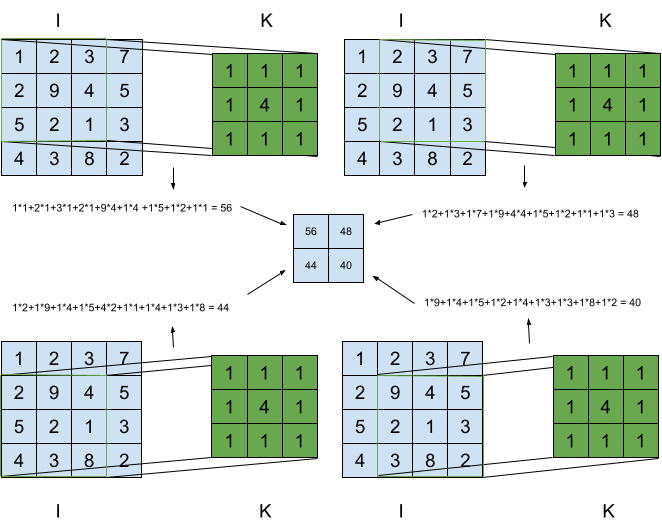
\includegraphics[scale=0.5]{Convolution.png}
    \centering    
    \caption{Illustration of discrete two dimensional convolution}
    \label{fig:Convolution}
\end{figure}

In practice, the convolution operation used in machine learning often corresponds to cross-correlation rather than strict mathematical convolution, differing by a sign flip in the kernel arguments. While this makes the operation non-commutative, it does not affect the learning process, as the learned kernel parameters will be equivalent \cite{deeplearningbook}.\newline


In digital signal processing, discrete convolutions are widely used with predefined kernels to manipulate signals predictably. Common examples include Gaussian kernels for blurring and edge detection kernels for highlighting areas of high intensity change. Figure \ref{fig:kernelIllustration} demonstrates the effects of these kernels. Edge detection provides insight into how CNNs learn features from data. In convolutional layers, kernels are learned to produce feature maps that aid in achieving the training objectives.
\begin{figure}[h]
    \centering
    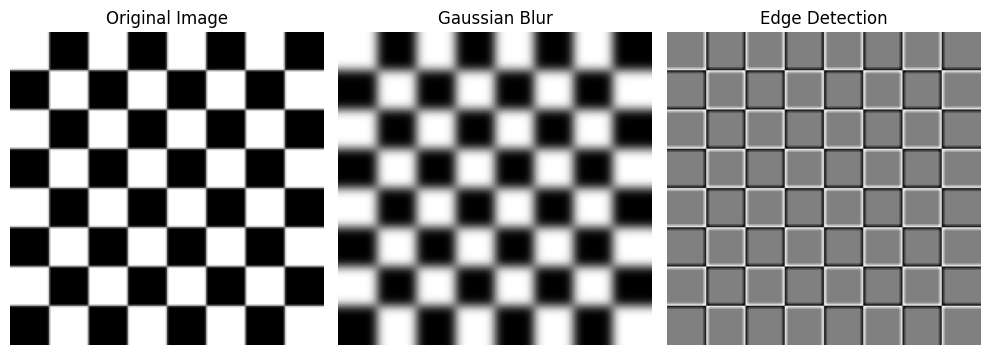
\includegraphics[scale = 0.5]{Kernel_illustration.png}
    \caption{Illustration of discrete convolution applied to images. Image part of Scikit-image data package.}
    \label{fig:kernelIllustration}
\end{figure}

\subsection{Pooling}
As mentioned earlier, CNNs are primarily used for high-dimensional data. To reduce the dimensionality to a manageable level, pooling operations are employed. Pooling is a downsampling technique applied to feature maps, where regions of the output are replaced with summary statistics. The aim with pooling is to retain the most important information while discarding less relevant details. Two of the most common pooling methods are max pooling and average pooling. Max pooling replaces the region with its maximum value, while average pooling replaces it with the average value.\newline

There are two key hyperparameters for any pooling operation: the filter size, which determines the region of values to calculate the summary statistic, and the stride length, which determines how the filter moves across the feature map. In addition to reducing dimensionality, pooling helps make representations approximately invariant to small distortions in the input. Illustrations of max pooling with different stride is presented in figure \ref{fig:mp2} and \ref{fig:mp2}, while the effect of max and average pooling on image data is illustrated in \ref{fig:mean_max_pool}.\newline

\begin{figure}[h]
    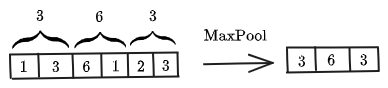
\includegraphics[scale=0.5]{MP_stride2}
    \centering    
    \caption{Max pooling of one dimensional array. Filter size: $2$, stride: $2$.}
    \label{fig:mp2}
\end{figure}
\begin{figure}[h]
    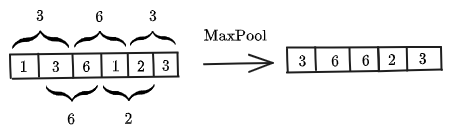
\includegraphics[scale=0.5]{MP_stride1}
    \centering    
    \caption{Max pooling of one dimensional array. Filter size: $2$, stride: $1$.}
    \label{fig:mp1}
\end{figure}

\begin{figure}[h]
    \centering
    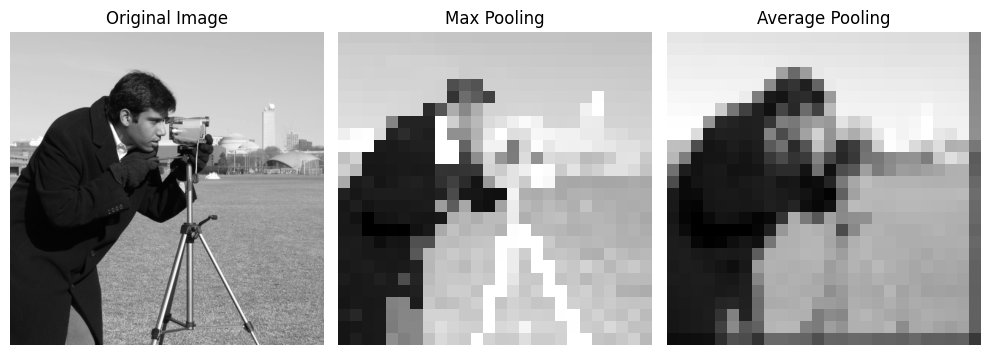
\includegraphics[scale = 0.5]{pooling_illustration.png}
    \caption{Illustration of mean and average pooling applied to images. Filter size and stride is $20\times 20$. Original image size is $512\times 512$, pooled images are $26\times26$. Image part of Scikit-image data package.}
    \label{fig:mean_max_pool}
\end{figure}

Global pooling is a technique that involves calculating a summary statistic, such as the maximum or average, for an entire feature map. This effectively summarizes the presence of a feature across the entire input. This method is particularly useful in the final layers of a convolutional neural network (CNN), where it reduces the spatial dimensions of the feature maps to a single value per map.

\subsection{Architecture}
There are many specific architectures within the category of convolutional neural networks (CNNs), but their basic components are largely the same. CNNs typically consist of convolutional layers, pooling layers, and fully connected layers. Figure \ref{fig:LeNet5} illustrates the original LeNet-5 \cite{LeCun1989ConvNet} as an example of a general CNN.\newline

\textbf{A convolutional layer} consists of several kernels. Each kernel is convolved with the entire input, producing the feature maps. After convolution, a nonlinear activation function is applied pointwise to the feature maps, introducing nonlinearity to the model. The purpose of the convolutional layer is to extract local features such as edges, textures, and shapes from the input data.
\begin{figure}[h]
    \centering
    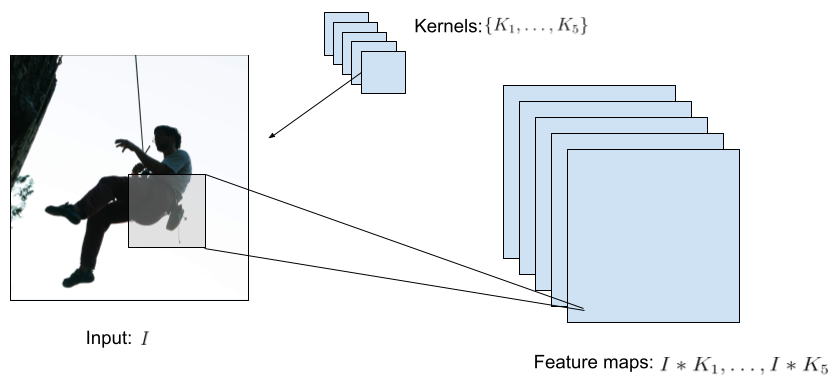
\includegraphics[scale = 0.5]{convlayer.png}
    \caption{Convolutional layer.}
    \label{fig:convlayer}
\end{figure}

\textbf{A pooling layer} is typically placed between convolutional layers and act as strong downsamplers that aim to enforce approximate translation invariance. A pooling operation, such as max pooling or average pooling, is applied across each feature map, reducing its dimensions while retaining important information. The pooling layer helps to reduce the computational load and control overfitting by progressively reducing the size of the representations.\newline

\textbf{Fully connected layers} are standard hidden layers in a neural network, connecting every input to every node in the output. Due to computational constraints, fully connected layers are introduced only after the input data has been sufficiently downsampled through convolutional and pooling layers. The fully connected layers aggregate the local features learned by convolutional layers, learning high level reasoning and enabling the network to make final classifications or predictions.\newline

\begin{figure}[h]
    \centering
    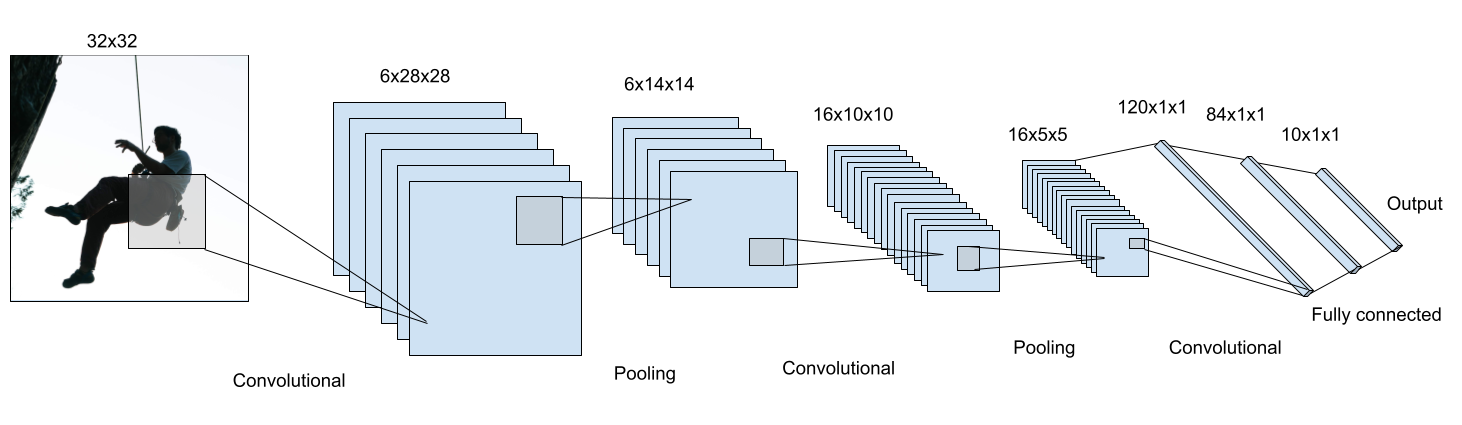
\includegraphics[scale = 0.25]{LeNet5.png}
    \caption{LeNet-5 network \cite{LeCun1989ConvNet}}
    \label{fig:LeNet5}
\end{figure}

In addition to these basic layers, modern CNN architectures often incorporate other techniques and layers to improve performance. Batch Normalization layers, for example, normalizes the inputs, which assist in stabilizing and speeding up the training process. They allow for higher learning rates and reduces the dependency on careful initialization.\newline

Additionally, residual connections are frequently used in modern architectures. Introduced by He et al. in \cite{he2015deep}, residual connections allow gradients to flow directly through the network, alleviating the vanishing gradient problem in deep networks \cite{279181}. They enable the training of much deeper networks by providing shortcut connections that bypass one or more layers. This means that instead of learning the underlying mapping directly, the network learns the residual function, which is often easier to optimize. Residual connections have been a key innovation, enabling the development of very deep networks like ResNet \cite{he2015deep}, which have achieved state-of-the-art results in various computer vision tasks.

\subsection{Transposed Convolutional Networks}
Transposed convolution, also known as deconvolution or fractionally-strided convolution, is a technique used to reverse the downsampling effect of convolutions. In essence, it is an inpainting or upsampling technique familiar from digital signal processing. The flexibility of learning data-dependent transposed convolutional kernels enables effective reversal of the downsampling performed by convolutional layers.\newline

Transposed convolutions are extensively used in combination with convolutional downsampling in encoder-decoder architectures presented in section \ref{section:VQVAE}. These architectures are fundamental in many generative models. The encoder part of the network typically reduces the dimensions through a series of convolutional and pooling layers, capturing the essential features of the input data. The decoder part then uses transposed convolutions to upsample the encoded feature maps back to the original dimensions, reconstructing the input or generating new data.\newline

\begin{figure}[h]
    \centering
    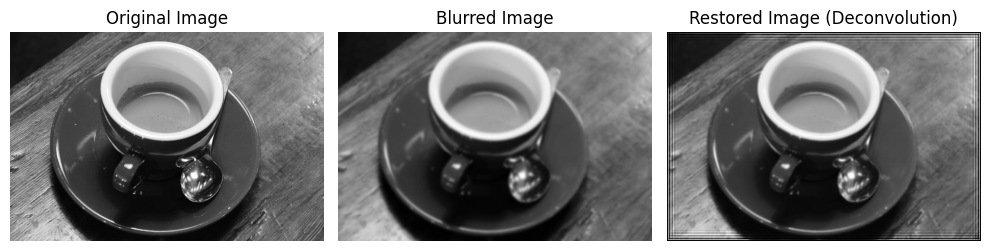
\includegraphics[scale = 0.5]{deconv_illustration.png}
    \caption{Illustration of deconvolution applied to images. Here using Gaussian blur and restoring using the Richardson Lucy algorithm with a Gaussian deconvolution kernel. Image part of Scikit-image data package.}
    \label{fig:deconv}
\end{figure}

Figure \ref{fig:deconv} illustrates the application of deconvolution to images. In this example, a Gaussian blur is applied, and the image is restored using the Richardson-Lucy algorithm with a Gaussian deconvolution kernel. This process demonstrates that transposed convolutions can be used to approximately reverse the effects of convolutional operations.


% \section{Residual Neural Network}

% Deep neural networks are hard to train. But we want deeper networks as the representations learned in deeper networks tend to be higher level/more abstract \cite{zeiler2013visualizing}. 

% The problem of exploding/vanishing gradients \todo{write about and explain what this is} has been to a large extent been solved by normalized initialization and intermediate normalization layers. This has enabled networks of tens of layers to start converging for SDG with backprop \cite{he2015deep}. \TODO{Rewrite the above in more of my own words}.



% The degeneration problem: 

% The deep residual learning framework was developed to address the degeneration problem.

% \cite{he2015deep}

% \section{Dimension reduction/visualization techniques}

% \subsection{PCA}
% Principle component analysis i a linear dimmension reduction technique which provides the axes of a point cloud 
%  PCA provides a linear projection on the eigenspace of the covariance matrix of the data. 



% \subsection{t-SNE}
% \cite{t-SNE}
% T distributed stochastic neighnourhood encoding.

% \subsection{UMAP}
% \cite{mcinnes2020umap}

% \subsubsection{densMAP}


\section{Representation Learning}

Representation learning is a term that can be difficult to define due to its abstract nature. To understand it better, let's first consider what is meant by the representation of information.\newline

Take the base ten integer $(4)_{10}= 4$ as an example. This number can be equivalently expressed in other base, such as binary $(4)_{2}=100$. The base we choose depends on our intention. For digital electronics, a binary representation is useful because transistors have two states. For human arithmetic, base ten is natural because we have ten fingers. Thus, a particular representation can make a task easier or harder, although the information content remains unchanged. What changes is the ease or difficulty of certain information processing tasks. Representation learning is the process of learning a representation of information that facilitates these tasks.\newline

Representations are highly dependent on who or what will process the information. Consider the example of time. Humans have developed a standardized system for writing timestamps that works well for us. However, if we want to model time-dependent phenomena using tabular data, the DateTime representation might be unhelpful to a tree-based model. The numerical representation of timestamps close in time is not necessarily close in numerical value, such as 23:59 and 00:00. A possible solution is to change the representation to reflect the periodic nature of time by mapping it to a circle. This new representation might be less intuitive for humans but more useful to a computer.\newline

In machine learning, representation learning involves designing algorithms that learn representations useful for a specific objective. The goal is to find representations that make it easier for the machine learning models to process and understand the data, improving performance on the given tasks.

\subsection{Why do we care about representation learning?}
Those who has worked with data science or machine learning and has come across feature engineering are familiar the effect good feature engineering has on a models performance. The same people too knows the level of domain expertise, creativity and time is needed to feature engineer well. In reality much of the actual time spent in the process of deploying machine learning methods revolves around constructing good data pipelines and applying transformations that produce representations beneficial for the algorithm at hand \cite{Rep-rev-persp}. Thus the ability to automate such tasks would be incredibly beneficial, and ease the use of ML algorithms significantly. It is here one of the intriguing and promising features of neural networks, with its many specializations and architectures, comes into play. They have shown the ability to learn useful abstract representations of the data and provide automatic feature engineering \cite{Rep-rev-persp}. 


\subsection{What is a good representation?}

The quality of a representation is determined by how effectively it facilitates subsequent tasks. The idea of universally good representations is ill-defined because any representation derived from a non-invertible function can be specifically countered by designing a \textit{downstream tasks} that relies on the lost information, leading to poor performance. In essence, there is no free lunch in representation learning either.\newline

To evaluate the quality of a representation, one must specify a set of predefined downstream tasks and assess performance based on those tasks. A representation is considered better if it enables the model to perform well on the downstream tasks. Additionally the more general a representation is, meaning they facilitate high performance on a larger set of tasks, the higher its quality.

\subsection{How does one evaluate representations?}
There are several evaluation protocols in representation learning. These typically involve training a model on a \textit{pretext task}, which, as defined in \cite{jing2019selfsupervised}, is a task designed for the network to solve with the primary goal of learning useful representations. The learned representations are then evaluated on a downstream task, generally solved in a supervised manner using human-annotated data.\newline

In an $N$-layered network $f = f_N\circ ...\circ f_1$, the intermediate value of the data $x$ in some layer $n$ represents the network's learned feature representations. When focusing on the learned representations, it is helpful to decompose the model $f$, notation wise, into a \textit{feature extractor} $h$ and an \textit{output function} $g$ such that it can be factored as $f = g \circ h$. Representation learning algorithms typically follow this pattern
\begin{itemize}
    \item Train $f= g \circ h$ on a pretext task.
    \item Discard $g$
    \item Use the learned feature extractor $\widehat{h}$ as part of a new model.
    \item Evaluate the new model on the downstream task. 
\end{itemize}

The standard evaluation protocol involves training a linear head $g_D$ on top of the \textit{frozen} representations in a supervised manner and evaluate this model's performance. This means training $f_D = g_D\circ \widehat{h}$ by only updating the parameters of the linear layer $g_D$, and evaluate $\widehat{f}_D$ on a test set. This protocol is sometimes referred to as \textit{linear probing}. A common downstream task is classification, where the idea is that good and informative representations should differentiate data in such a way that it is easy to separate them. \newline

An alternative protocol, similar to the one above, allows all parameters of $f_D$ to be learnable on the downstream task. This protocol is referred to as a pretraining-finetuning. In this approach, the model typically is pretrained on a large, potentially unlabeled dataset, and then fine-tuned on a smaller, labeled dataset specific to the downstream task. \newline

Evaluating $f_D$ involves assessing accuracy on the downstream task, training time, and the sensitivity of these metrics to the training data size. The baseline comparison is typically an identical but randomly initialized model. It is highly advantageous if one can pretrain a feature extractor using abundant, cheap data, ensuring faster convergence on a downstream task where data is expensive or scarce.\newline

It is worth mentioning that in cases where the sole goal is to create the best-performing model, a more complex task-specific head $g_D$ is often used. For a comprehensive survey on representation learning, see\cite{nozawa2022empirical}.


\begin{figure}[h]
    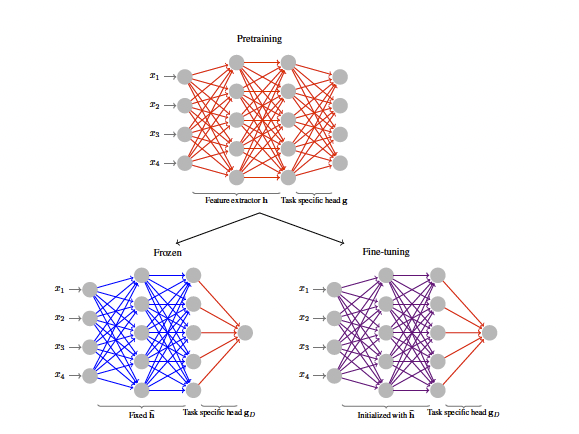
\includegraphics[scale=0.5]{rep_learnin_protocol.png}
    \centering    
    \caption{Taken from \cite{nozawa2022empirical}}
\end{figure}


\section{Transformers}

Since their introduction in the seminal paper "Attention is all you need"\cite{vaswani2023attention}, transformers have revolutionized the fields of machine learning and artificial intelligence. This architecture is the backbone of large language models (LLMs) such as Google's BERT, Meta's Llama and OpenAI's ChatGPT. Following their initial success in natural language processing, transformers have been adapted for other modalities, including computer vision with Vision Transformers \cite{dosovitskiy2021image}, and similar trends are shown for other modalities such as audio \cite{latif2023transformers} and time series \cite{wen2023transformers}. \newline

Transformers were developed for sequential modeling and have the capability of learning long-range dependencies in data through the \textit{multi-headed attention mechanism}.  Previously, recurrent neural networks (RNNs) and long short-term memory (LSTM) networks were the state-of-the-art for sequential tasks. However, they struggled with modeling long-term dependencies due to the vanishing or exploding gradient problem \cite{279181}. One of the main novelties of the transformer architecture is not relying on recurrence, and instead solely using the attention mechanism to capture dependencies between input and output.
\newline

The transformer takes as input a sequence of symbols. For different modalities like text, speech, images, and time series, this requires a process called \textit{tokenization}. For example, in natural language processing (NLP), a simple word-level tokenization involves creating a dictionary of all words in the dataset and assigning each word an integer. Text can then be mapped to a sequence of integers. Other modalities, such as speech, images, and time series, are usually represented as matrices which can be flattend and used as inpus. However, directly modeling high-dimensional data as such sequences would require significant computational resources and make it challenging to model long-range dependencies. Therefore, various tokenization methods are used to represent the data as coarser sequences. 
\newline

Transformers have also been successfully adopted for generative tasks. Autoregressive transformers, such as the GPT series, are trained to predict the next token in a sequence given the preceding tokens. By treating images as sequences of patches, Vision Transformers can generate new images or inpaint missing patches based on the input. With the introduction of Vision Transformers \cite{dosovitskiy2021image}, input images are split into patches and linearly projected before being processed by the transformer. Since then, \textit{Vector-Quantized}-based tokenization introduced by \cite{VQVAE} has emerged as a popular approach.

\subsection{The Attention Mechanism}

The attention mechanism is a key innovation in transformer architectures, enabling them to handle long-range dependencies effectively. Attention can be described as mapping a query and a set of key-value pairs to an output, where the query, keys, values, and outputs are all vectors. This mechanism allows the model to focus on different parts of the input sequence simultaneously.

\begin{figure}[h]
    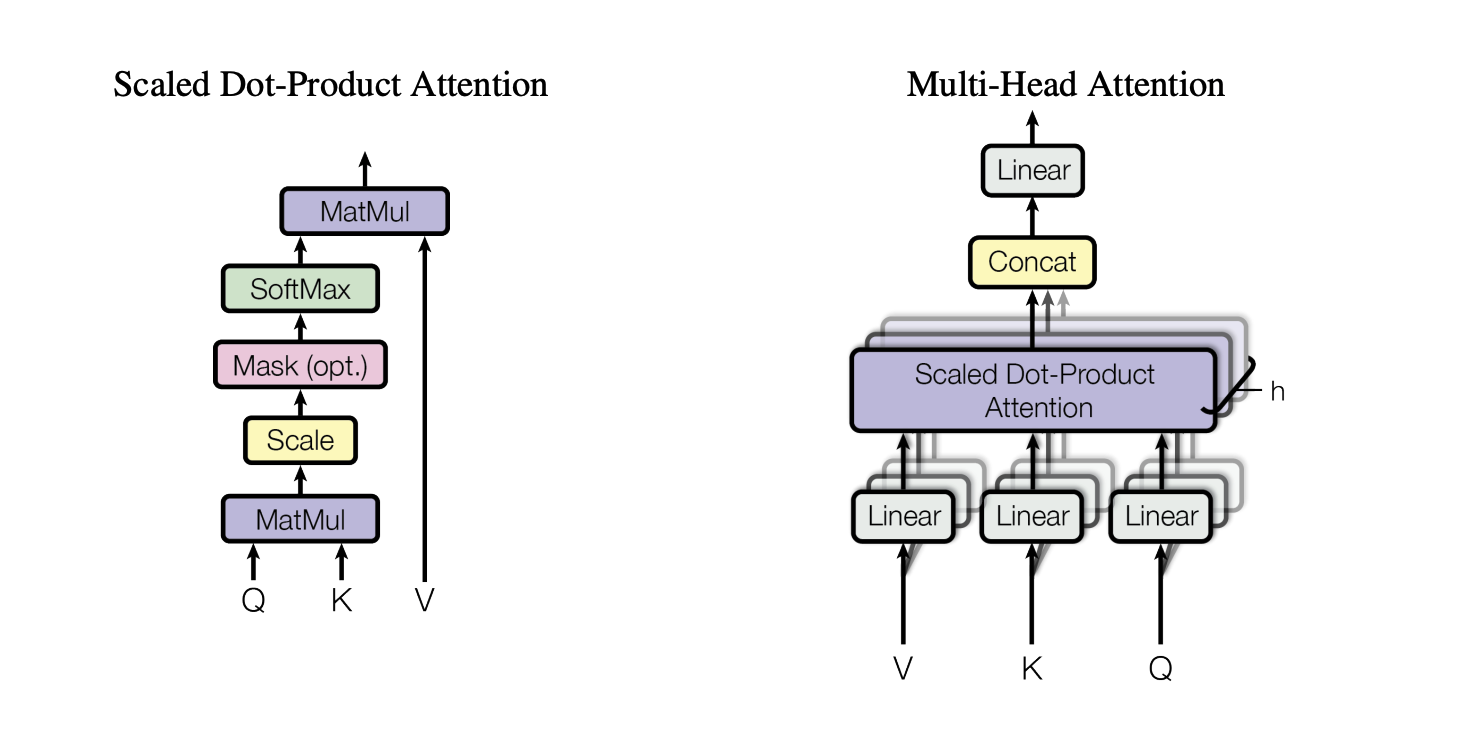
\includegraphics[scale=0.25]{Attention.png}
    \centering 
    \caption{(left) Scaled dot-product attention. (right) Multi-headed attention. Taken with permission from \cite{vaswani2023attention}}
    \label{fig:attention}
\end{figure}

Scaled dot-product attention is computed by 

\begin{equation}
    \text{Attention}(Q,K,V) = \softmax \left(\frac{QK^T}{\sqrt{d_k}}\right)V
\end{equation}

This equation allows the model to weigh the importance of different input tokens based on their relevance to the query, enabling it to focus on the most relevant parts of the input.\newline



To enhance the model's ability to capture different aspects of the input, multi-headed attention is used. This involves projecting the queries $Q$, keys $k$, and values $V$ into multiple subspaces and applying scaled dot-product attention in each subspace. The results from each subspace are then concatenated and linearly transformed. The process is defined as

\begin{equation}
    \text{MultiHead}(Q,K,V) = \text{Concat}(\text{head}_1,\dots, \text{head}_h)W^O,
\end{equation}
where
\begin{equation}
    \text{head}_i = \text{Attention}(QW_i^Q,KW_i^K,VW_i^V). 
\end{equation}

Multi-headed attention enables the transformer to attend to different parts of the input sequence and capture various features simultaneously. By having multiple attention heads, the model can learn different relationships and dependencies within the data, leading to richer representations.

\subsection{Architecture}

The original transformer architecture, as presented in Figure \ref{fig:transformer}, consists of several distinct components that work together to process sequential data effectively. This architecture includes an encoder and a decoder, each composed of multiple layers that leverage the attention mechanism to handle dependencies within the input data.\newline

\begin{figure}[h]
    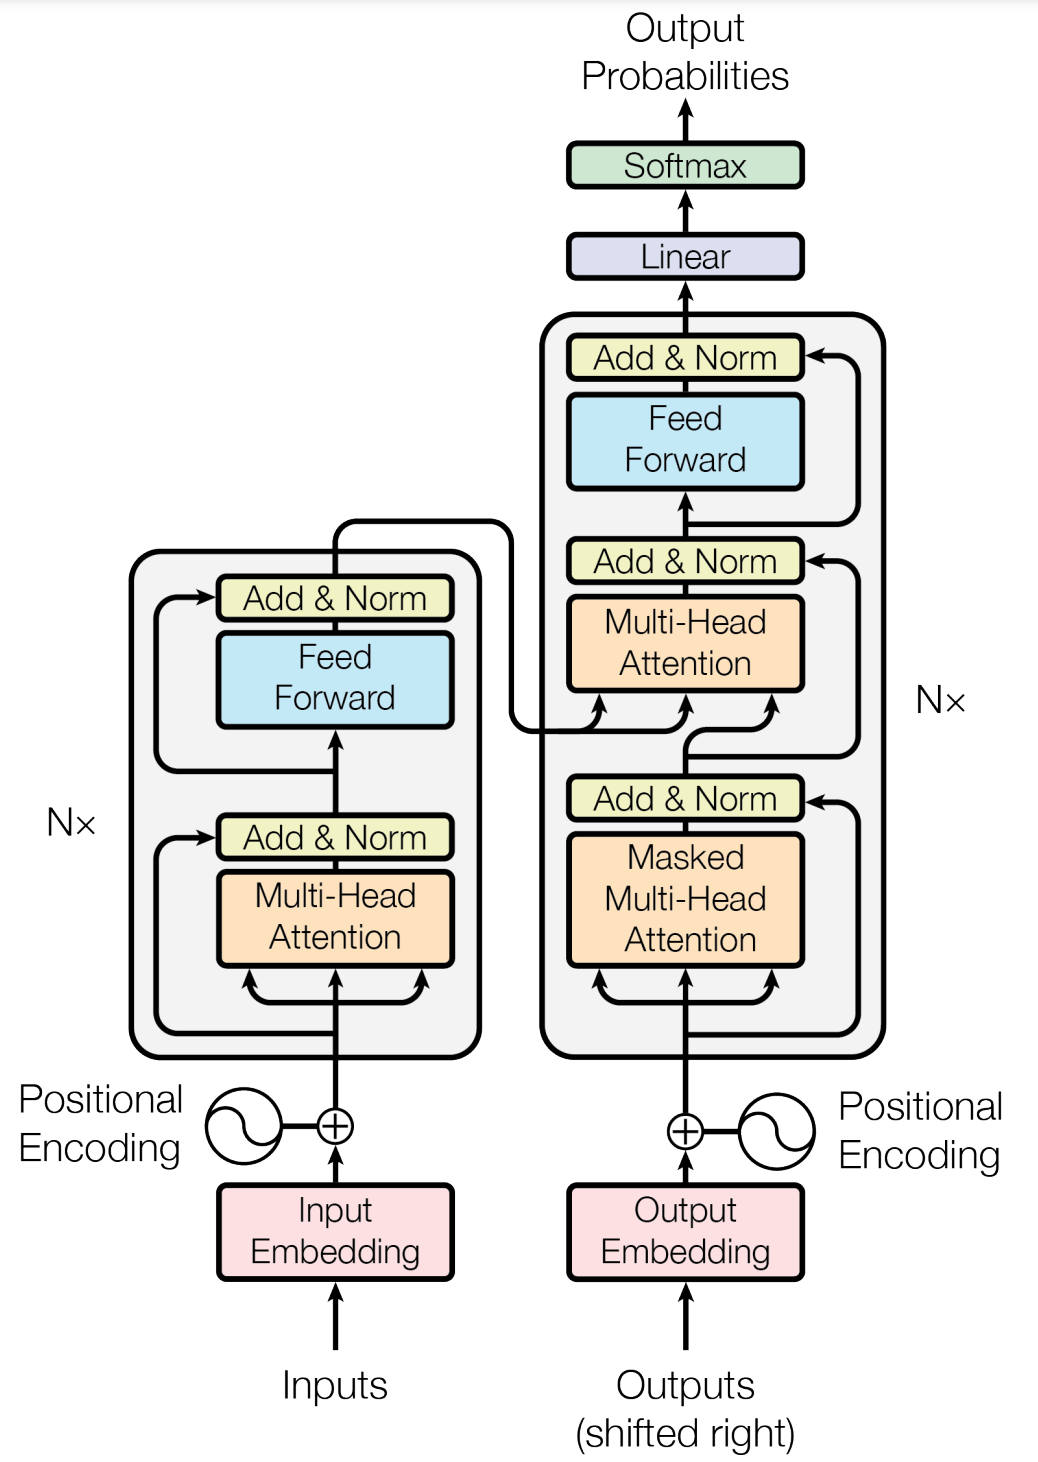
\includegraphics[scale=0.1]{Transformer_architecture}
    \centering 
    \caption{The Transformer - model architecture. Encoder (left), decoder (right). Taken with permission from \cite{vaswani2023attention}}
    \label{fig:transformer}
\end{figure}


\textbf{Embeddings}: The first step in the transformer architecture involves mapping each token in the input sequence to a vector through an input embedding. This process is essentially a lookup table where each token is converted into a continuous vector representation. These embeddings allow the model to process and learn from the input data more effectively.
\newline

\textbf{Positional encoding}: Transformers do not inherently account for the order of the input sequence, as they lack the sequential nature of recurrent models. To address this, positional encoding is added to the input embeddings. Positional encoding provides information about the position of each token in the sequence, allowing the model to differentiate between tokens based on their order. In the original paper \cite{vaswani2023attention}, sinusoidal functions were used to generate unique positional encodings for each position.
\newline

\textbf{Encoder}: The transformer encoder processes the input embeddings with positional encodings through multiple identical layers. Each encoder layer consists of two main components. The multi-head attention layer enables the model to focus on different parts of the input sequence simultaneously, capturing various dependencies. This is followed by a fully connected layer which processes the output of the multi-head attention, further transforming the data. Each sublayer incorporates residual connections and normalization. 
\newline

\textbf{Decoder}: The transformer decoder is similarly structured, consisting of multiple identical layers. They consist of a masked attention layer, which is similar to an attetion layer but prevents the model from attending to future tokens in the sequence during training, ensuring that predictions are based only on past and present tokens. A multi-head attention which is applied to the output of the encoder and a fully connected neural network. All sublayers employ residual connections and normalization. The final output of the decoder is converted to probabilities using a linear layer followed by a softmax function.
\newline

Bidirectional transformer models, such as BERT \cite{devlin2019bert}, utilize an encoder-only architecture. This design allows the attention mechanism to consider information from both directions within the sequence, enabling the model to capture a more comprehensive understanding of the context. The issue of "seeing into the future" is resolved through a training technique called \textit{masked modeling}, where some tokens are masked and the model is trained to predict them based on the surrounding context. This will be looked at further in Section \ref{section:Masked modelling}.

\section{Self-Supervised learning}

Self-supervised learning (SSL) has achieved great success in natural language processing (NLP) and computer vision in recent years and is rapidly being applied to other modalities. In our work, we leverage SSL for representation learning in the time series domain. Before diving into SSL, it is important to understand the broader context of machine learning, which can be coarsely divided into two categories: supervised and unsupervised learning.
\newline

\subsubsection*{Supervised Learning}

Supervised learning involves training models using labeled data. For a given input $x$, the desired output $y$ is known during training, allowing for direct supervision of the model's parameters by comparing its output to the true value. A bit more formally, for a dataset $X = \{x_i\}_{i=1}^N$ with corresponding human-annotated labels $Y = \{y_i\}_{i=1}^N$, the objective of a supervised learning algorithm is to fit a function $f_\theta$ that minimizes the loss across the data
\begin{equation}
    \widehat{f}_\theta = \min_\theta \frac{1}{N} \sum_{i=1}^N L(f_\theta(x_i),y_i).
\end{equation}

Common approaches to supervised learning for neural networks is to calculate some distance metric between the predicted value $\widehat{y}$ and the true value $y$ and update parameters using backpropagation.\newline

Supervised learning models, including classical statistical models, support vector machines, and decision tree-based models, have seen tremendous success but are limited by the need for labeled data, which is often scarce and expensive to obtain.

\subsubsection*{Unsupervised Learning}

Unsupervised learning, on the other hand, refers to models that learn exclusively from unlabeled data, discovering intrinsic patterns without explicit labels. Examples of unsupervised learning techniques include clustering methods (e.g., K-means, K Nearest Neighbor, Gaussian mixture models), dimensionality reduction techniques (e.g., PCA, SVD), and neural network architectures such as autoencoders. These techniques are widely used in exploratory data analysis, data visualization, and clustering. While unsupervised learning is valuable in a world abundant with unlabeled data, it has historically struggled to match the performance of supervised approaches.

\subsubsection*{Self-Supervised Learning}

Self-supervised learning is a subcategory of unsupervised learning that has shown remarkable success in NLP and computer vision, approaching the performance of state-of-the-art supervised representation learning \cite{bardes2022vicreg, zbontar2021barlow}. SSL involves using the data itself to generate a supervisory signal, rather than relying on external labels. Although SSL is technically unsupervised, its learning formulation closely resembles that of supervised learning.\newline

For a dataset $X = \{x_i\}_{i=1}^N$ with \textit{pseudo labels} $P = \{p_i\}_{i=1}^N$, the objective of a self-supervised learning algorithm is to fit a function $f_\theta$ hat minimizes the loss across the data
\begin{equation}
    \widehat{f}_\theta = \min_\theta \frac{1}{N} \sum_{i=1}^N L(f_\theta(x_i),p_i).
\end{equation}

Pseudo labels are automatically generated labels from the data. In \textit{siamese} architectures, these pseudo labels are typically augmentations of the original data. SSL has become an integral part of pretraining large models, enabling them to learn from vast amounts of unlabeled data. Pretraining with SSL allows models to capture the semantics of data without the need for extensive labeled datasets, significantly reducing the resources required for subsequent supervised training.

\subsection{Siamese Architecture-based SSL }
A siamese network architecture \cite{siamese} consists of two branches with a shared encoder on each branch. These networks are trained to produce similar representations for different views of the same data. A major challenge in this architecture is avoiding trivial solutions, where the networks ignore the input and produce identical constant embeddings, a problem known as \textit{collapse}.\newline
\TODO{Figure of siamese}

In computer vision, several representation learning algorithms utilizing siamese architectures have been proposed. These can be broadly categorized into \textit{contrastive} and \textit{non-contrastive} SSL methods.\newline

Contrastive SSL uses positive and negative samples to learn representations by pulling positive pairs closer together and pushing negative pairs further apart. Examples include MoCo \cite{he2020momentum} and SimCLR \cite{chen2020simple}. Contrastive methods often require large batch sizes as well as a substatial number of negative pairs compared to positive in order to learn representations effectively \cite{lee2024computer}.\newline

Non-Contrastive SSL methods, such as BYOL \cite{grill2020bootstrap}, BarlowTwins \cite{zbontar2021barlow} and VIbCReg \cite{lee2024computer} avoid the need for positive and negative pairs. These methods use augmentations of the input data as pseudo labels and introduce different mechanisms to prevent collapse. For instance, BYOL introduces architectural asymmetry and the stop-gradient operation, Barlow Twins minimizes information redundancy between branches, and VICReg maintains variability while decorrelating features in each branch.

\subsubsection{Projector}

Most siamese architecture-based self-supervised learning (SSL) methods utilize a projector to produce embeddings for the SSL loss. A projector is a neural network designed to map representations onto a subspace or expand them into a larger space, depending on the SSL method. In the literature, some differentiate between projection networks (projectors) and expanding networks (expanders). However, in our work, we use VICReg and Barlow Twins, both of which utilize expanding networks as projectors. For considerations on low-rank projectors, refer to \cite{gupta2022understanding}.\newline

Similar to the setup described in the representation learning section, we can view the projector as a head $g$ in the model $f = g\circ h$, with the output of $h$ considered as the representations. The primary reason for not using the projector's output as our representations is that these embeddings are too specialized for minimizing the SSL loss and generalize poorly. While the exact reasons for this behavior are unclear, empirical results consistently show the superiority of using the projector's input rather than its output for downstream tasks.\newline

Experiments on the architecture of expanding projectors, simply referred to as projectors, in \cite{zbontar2021barlow,bardes2022vicreg} indicate a steady performance gain when increasing the projector's width (output dimension) from 256 to 8192. However, performance saturates when the depth (number of layers) reaches three.\newline

Projectors used in SSL methods that employ variance/covariance regularization, such as Barlow Twins and VIbCReg, help enforce pairwise independence of the components of representations \cite{mialon2024variance}. Independent representation features is in the literature considered a desired property, though not universally accepted \cite{träuble2021disentangled,Rep-rev-persp}. The article \cite{mialon2024variance} attempt to explain why shallow and wide projectors typically result in improved representations. The main argument is that, as stated in Lemma 2, when the projector has orthogonal weights, minimizing the covariance of the projector output amounts to minimizing the pairwise correlation of the input components. For wider projectors, the orthogonality assumption is more accurate, as the dot product of randomly initialized vectors with zero mean tends to zero as the dimension increases, by the central limit theorem. They further argue that learning the projector is only crucial for maintaining variability, and that for wider networks, the weights need not move far from the random initialization to successfully maintain variance.   

\subsection{Masked modelling}
\label{section:Masked modelling}
Masked modeling is a straightforward self-supervised learning technique for generative models. The core idea is to mask or cover a portion of the data and train the model to predict the masked portions. By comparing the predictions against the unmasked data, the model learns useful representations without explicit supervision. Introduced in NLP by BERT \cite{devlin2019bert}, masked modeling has become the standard for self-supervised pretraining of language models.\newline

In computer vision, masked modeling has also gained attention. Initial approaches involved masking image patches directly \cite{he2021masked}. With the success of vision transformers \cite{dosovitskiy2021image}, researchers began tokenizing images and pretraining transformers in a manner similar to BERT. For example, MaskGIT \cite{chang2022maskgit} proposed masked visual token modeling, using vector-quantized-based tokenization and a bidirectional transformer. For a comprehensive survey on masked modeling in the vision domain, refer to \cite{li2024masked}.

\section{Vector Quantized Variational Autoencoder (VQVAE)}
\label{section:VQVAE}
Our model is based on the Vector Quantized Variational Autoencoder (VQVAE) introduced in \cite{VQVAE}, and includes an Autoencoder (AE) branch. Therefore it is natural to dive into the models. We first start with introducing autoencoders, then present the variational variation VAE before presenting VQVAE. 

\subsection{Autoencoder (AE)}

An autoencoder consists of two neural networks: an encoder $E$ and a decoder $D$. These networks map data between two spaces: the data space $X$ and the latent space $Z$. The encoder compresses the data from the data space to the latent space, while the decoder reconstructs the data from the latent space back to the data space. A schematic of the architecture is presented in Figure \ref{fig:autoencoder}. \newline

\begin{figure}[h]
    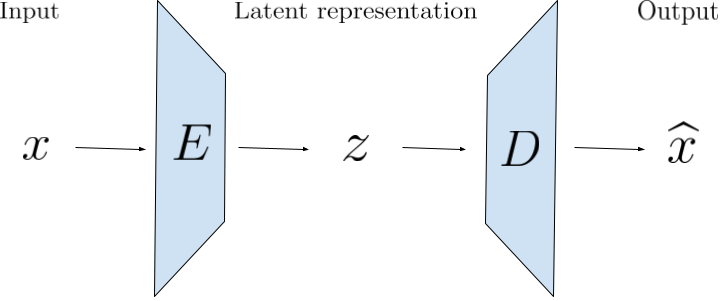
\includegraphics[scale = 0.3]{Autoencoder.png}
    \centering
    \caption{Schematics of the autoencoder architecture.}
    \label{fig:autoencoder}
\end{figure}

The primary goal of an autoencoder is to learn an efficient encoding of the data. The encoder compresses the data into a lower-dimensional representation, and the decoder reconstructs the original data from this compressed representation. The training objective is to make the composition of the encoder and decoder approximate the identity function, meaning that the output should be as close as possible to the input. Autoencoders are typically trained to minimize the reconstruction error, which typically is the mean square error (MSE) between the input and the reconstructed output. This process forces the model to learn efficient latent representations of the data.\newline

One of the critical aspects of autoencoders is the \textit{information bottleneck}. The dimension of the latent space is much smaller than that of the data space. This bottleneck forces the model to capture the most important features of the data while discarding less relevant information. By compressing the data, the encoder learns a compact representation that retains the essential features needed for accurate reconstruction by the decoder. However, learning effective latent representations can be challenging. Without proper regularization, the latent space may capture noise or irrelevant details, leading to overfitting.\newline

Event though Autoencoders are outdated, they serve as the foundational building block for more complex models such as Variational Autoencoders (VAEs) and Vector Quantized Variational Autoencoders (VQVAEs), which further enhance the ability to learn meaningful and useful representations from data.

\subsection{Variational Autoencoder (VAE)}
Variational Autoencoders (VAE) were introduced in \cite{kingma2022autoencoding} and is a variational Bayes approach to approximate inference and learning with directed probabilistic models. While the architecture of VAEs, presented in Figure \ref{fig:VAE_Normal}, is similar to that of traditional autoencoders, their mathematical formulation is fundamentally different. Variational inference is a statistical technique used to approximate complex distributions by finding the closest approximation within a simpler, but flexible, parametric family. \newline 

In the VAE framework, we assume that the dataset $X = \{x_i\}_{i=1}^{N}$ consists of iid samples from a random variable $\mathbf{x}$. We further assume that the data is generated by some unobservable random process. Specifically, that there is a latent variable $\mathbf{z}$ such that $x_i \sim p_{\theta^*}(x|z_i)$, where $z_i \sim p_{\theta^*}(z)$. The distribution $p_{\theta^*}(z)$ is referred to at the true prior, and $p_{\theta^*}(x|z_i)$ as the true likelihood. Since $\mathbf{z}$ is unobservable and the true distributions are unknown, one has to assume their form. In general the prior and likelihood are assumed to be from parametric families $p_{\theta}(z)$ and $p_{\theta}(x|z)$. These distributions are typically chosen to be differentiable to facilitate gradient-based learning.\newline
% \begin{figure}[h]
%     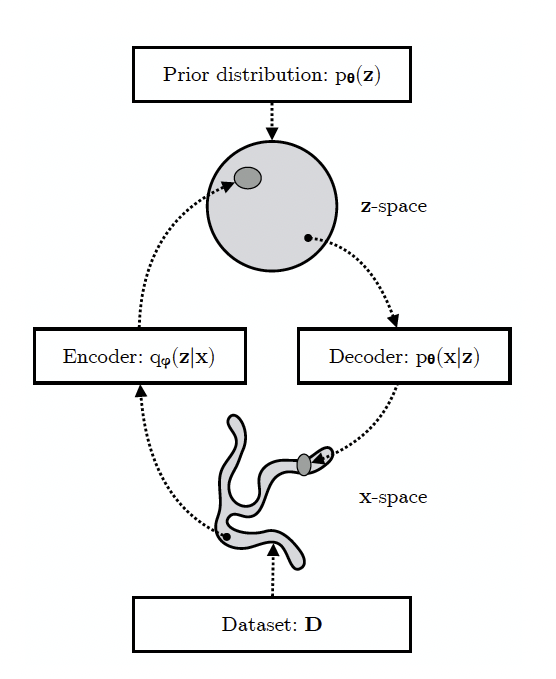
\includegraphics[scale=0.3]{VAE}
%     \centering  
%     \caption{\cite{VAE}, need to ask for permission or make own}  
% \end{figure}

VAEs have two main components: the probabilistic encoder (or inference model) $q_\phi(z|x)$, which approximates the true posterior, and the probabilistic decoder (or generative model) $p_\theta(x|z)$, which approximates the likelihood. These models are typically parameterized by neural networks, with $\phi$ and $\theta$ representing their weights and biases. Given a datapoint $x_i$, the probabilistic encoder provides a distribution over the possible values of the latent variable $\mathbf{z}$. Similarly, given a latent representation $z_i$, the probabilistic decoder produces a distribution over the possible corresponding values of $\mathbf{x}$. \newline

The probabilistic nature of the encoder and decoder involves sampling. For a given $x$ or $z$, the output is a distribution, and the same input will yield the same output distribution if the network parameters are unchanged. Actually, $x$ and $z$ are mapped to the parameters of a distribution, which uniquely determines the distribution in a particular family.\newline

Common assumptions for the distributions are:
\begin{itemize}
    \item Prior $p_\theta(z)\sim N(0,I)$
    \item Likelihood $p_\theta(x|z)\sim N(D(z), I)$
    \item Variational posterior $q_\phi(z|x)\sim N(E(x)) = N(\mu_x, \Sigma_x)$
\end{itemize}
The encoder maps datapoints to the parameters of the variational distribution $q_\phi$, 
$$x \mapsto E(x) = (\mu_x, \Sigma_x).$$ 
A latent representation $z$ is then sampled from $q_\phi$, which constitutes the random part of the algorithm. The decoder maps $z$ to the expected value of the likelihood $p(x|z)$, 
$$z \mapsto D(z) = \widehat{x}.$$ 

There are several reasons for choosing Gaussian distributions, one being that the Gaussian distribution a scale-location family. This enables us to employ the reparameterization trick, and circumvent the problematic random component in the VAE when using gradient based learning. It involves introducing an auxillary variable $\epsilon \sim N(0,I)$ and rewriting $z = \mu_x + L_x\epsilon $, where $L_x$ is the Cholesky decomposition of $\Sigma_x$. This allows the gradient to flow through the deterministic parts of the model.
\begin{figure}[h]
    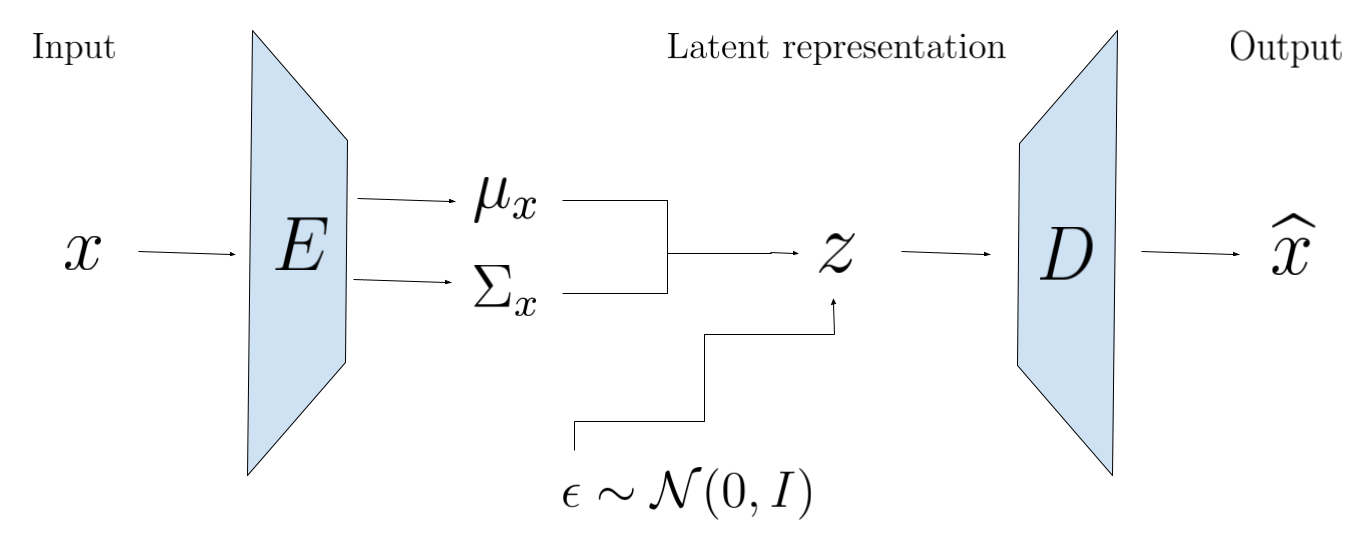
\includegraphics[scale = 0.2]{VAE_Normal.png}
    \centering
    \caption{Schematics of the VAE architecture with Gaussian reparameterization.}
    \label{fig:VAE_Normal}
\end{figure}


\subsubsection{Training objective}

VAEs are optimized with respect to the \textit{evidence lower bound} (ELBO). For jointly distributed variables $\x$ and $\z$ with distribution $p_\theta$. Then for any distribution $q_\phi$ the ELBO is defined as

\begin{equation}
    \label{eq:ELBO}
    \loss_{\theta,\phi}(x) 
    = \mathbb{E}_{q_\phi(z|x)} \log \left( \frac{p_\theta(x,z)}{q_\phi(z|x)}\right)
\end{equation}
This can be reformulated in terms of the marginal likelihood and KL divergence between the variational and true posterior
\begin{equation}
    \begin{aligned}
        \label{eq:ELBO_loglik}
        \loss_{\theta,\phi}(x) 
        &=  \mathbb{E}_{q_\phi(z|x)} \log \left( p_\theta(x)\right) + \mathbb{E}_{q_\phi(z|x)} \log \left( \frac{p_\theta(z|x)}{q_\phi(z|x)}\right) \\
        &= \log \left( p_\theta(x)\right) - \textrm{KL}(q_\phi(z|x)|| p_\theta(z|x)).
    \end{aligned}
\end{equation}

Due to the non-negativity of the KL-divergence, we see that the ELBO bounds the marginal log likelihood of the data from below. By maximizing the ELBO with respect to the model parameters $\phi$ and $\theta$,  one simultaneously maximizes the marginal likelihood and minimizes the KL divergence, improving both the generative and inference models \cite{VAE}.\newline

An alternative formulation shows a more evident connection to autoencoders, with the prior acting as a regularizer on the posterior
\begin{equation}
    \begin{aligned}
        \label{eq:ELBO_AE}
        \loss_{\theta,\phi}(x) 
        &=  \mathbb{E}_{q_\phi(z|x)} \log \left( p_\theta(x|z)\right) - \mathbb{E}_{q_\phi(z|x)} \log \left( \frac{q_\theta(z|x)}{p_\phi(z)}\right) \\
        &= \underbrace{\mathbb{E}_{q_\phi(z|x)} \log \left( p_\theta(x|z)\right)}_{\text{Expected reconstruction log likelihood}} - \underbrace{\textrm{KL}(q_\phi(z|x)|| p_\theta(z))}_{\text{Regularizer}}.
    \end{aligned}
\end{equation}

Assuming a Gaussian likelihood, we have

\begin{equation}
    \log p_\theta(x|z) = -\frac12 \left[k\log(2\pi)+ (x-\widehat{x})^T(x-\widehat{x})\right],
\end{equation}
which is equivalent, as an optimization objective of $\widehat{x}$, to $||x-\widehat{x}||_2^2$. Consequently the likelihood in the loss is implemented as the MSE of the input $x$ and the output $\widehat{x}$.

\subsubsection{Generative model}
The prior in a VAE serves two main roles: as a regularizing constraint for the posterior during training, and as a means of generating new samples via ancestral sampling. Ancestral sampling refers to $\z$ being the parent node of $\x$ in the VAE, and that we can generate samples $x$ by drawing a sample $z\sim p(z)$ and decode $D(z)$. 


\subsubsection{Limitations}

Despite their strengths, VAEs can suffer from issues such as posterior collapse, where the latent variable $\z$ fails to capture meaningful information about the input data. This can lead to poor reconstruction quality and less informative latent representations. Additionally, VAEs may struggle with variance issues, where the variance of the learned latent distributions is not well-calibrated, affecting the quality of generated samples.\newline

These limitations have motivated the development of more advanced models, such as the Vector Quantized Variational Autoencoder (VQVAE), which aims to address some of these challenges by introducing discrete latent variables and a learnable prior distribution.

% \subsection{Vector Quantization (VQ)}
% Dictionary learning model \cite{Gray1984VQ}

\subsection{VQVAE}
The Vector Quantized Variational Autoencoder (VQVAE) was first introduced in \cite{VQVAE} and presented a novel approach to training VAEs with discrete latent variables. It was the first model to achieve similar performance to continuous VAEs while utilizing discrete latent representations. VQVAE was developed to enhance representation learning by allowing the encoder network to output discrete codes and by learning the prior distribution rather than assuming it to be static. This approach provides more flexibility in capturing the underlying data distribution while simultaneously avoiding posterior collapse and variance issues observed in VAEs.

% \TODO{What do we gain by having a flexible posterior and a non-informative prior during training? The advantages for generative modelling to have a learnable prior? VAEs are traditionally quite bad when it comes to generative quality (sharpness). The flexibility of VQVAE seems to set the stage for better sample generation.}


\subsubsection{Architecture}

The overall architecture of VQVAE comprises three main components: an encoder, a decoder, and a \textit{codebook}. The encoder and decoder function similarly to those in traditional autoencoders, while the codebook, also referred to as the latent embedding space, acts as a lookup table for vector quantization.\newline

The codebook, denoted by $\mathcal{Z} = \{z_k\}_{i=1}^K$, consists of $K$ latent vectors with dimensionality $D$. During the encoding process, the output of the encoder $E(x)$ is quantized by finding the nearest neighbor in the codebook
\begin{equation}
    z_q = \argmin_{z_k\in\mathcal{Z}} ||E(x)-z_k||.
\end{equation}

\begin{figure}[h]
    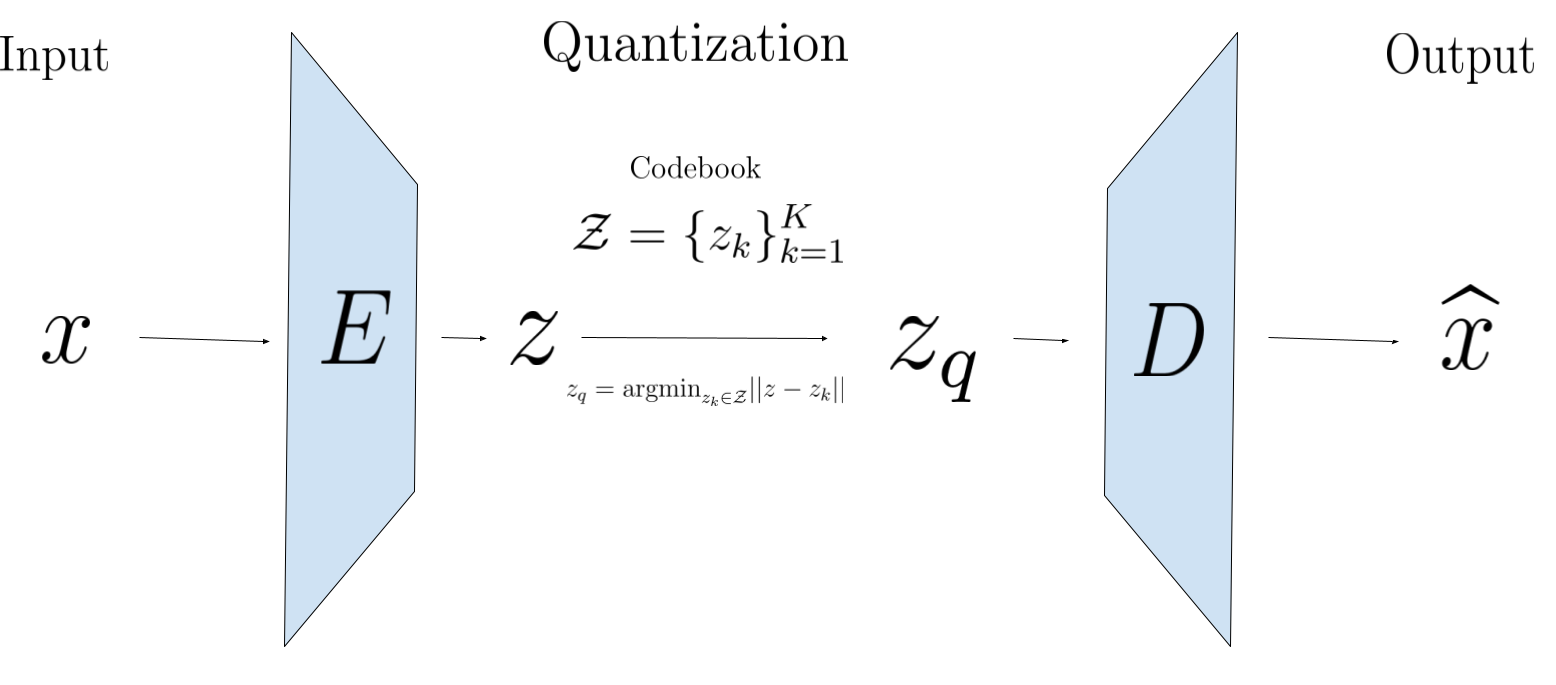
\includegraphics[scale = 0.2]{VQVAE.png}
    \centering
    \caption{Schematics of the VQVAE architecture.}
    \label{fig:VQVAE}
\end{figure}
From \ref{fig:VQVAE} we can see that the VQVAE can be seen as an autoencoder with a nonlinearity introduced by the vector quantization.

\subsubsection{ELBO}
Unlike traditional VAEs, where the posterior distribution is assumed to be Gaussian, the posterior in VQVAE is categorical. The probabilities are defined as
\begin{equation}
    p(z=k | x) = 
    \begin{cases} 
        1 \quad \text{for }k = \argmin_j||E(x) - z_j||_2 \\
        0 \quad \text{otherwise}
    \end{cases},
\end{equation}
Sampling from the posterior amounts to quantizing the output of the encoder, as it is deterministic. \newline

In the original article \cite{VQVAE}, the authors propose to learn the prior distribution separately after training the encoder, decoder, and codebook. Initially, the prior is assumed to be uniform, allowing the posterior to learn without constraints. The VQVAE can too be viewed as a VAE, allowing the use of the ELBO \ref{eq:ELBO_AE} to bound the marginal likelihood. Since the variational posterior is deterministic and the prior (during training) is uniform over $\{1,...,K\}$ we get that the regularizing term simplifies to a constant

\begin{equation}
    \begin{aligned}
        \KL(q(z|x)||p(z)) &= \sum_{z}  q(z|x) \log \left(\frac{q(z|x)}{p(z)}\right) \\
                           &= q(z=k|x) \log \left(\frac{q(z=k|x)}{p(z=k)}\right) \text{, $q$ is deterministic}\\
                           &= \log \left(\frac{1}{1/K}\right) \text{, uniform prior}\\
                           &= \log(K).
    \end{aligned}
\end{equation}
Thus, the ELBO reduces to the reconstruction term only.

\subsubsection{Loss funciton}
\label{section:VQVAELoss}
The VQVAE employs a loss function designed to facilitate gradient-based learning despite the non-continuous nature of the quantization process. As the input of the decoder has the same dimension, we circumvent the discontinuities by simply copying the gradients from the decoder to the encoder. The gradients from the decoder contains relevant information to how the encoder should change its output, and in the subsequent forward pass the encoder output can be quantized to different discrete latent codes.\newline


The overall loss function in VQVAE consists of two main components, the reconstruction loss and the codebook loss. The reconstruction loss ensures that the output of the decoder closely matches the input, while the codebook loss manages the relationship between the encoder output and the quantized output.\newline

The reconstruction loss is the typical mean square error of the input $x$ and the reconstructed output $\widehat{x}$
\begin{equation}
    \loss_{\text{recons}} = ||x - \widehat{x}||_2^2.
\end{equation}

The codebook loss has two parts. The first part measures the euclidean distance between the encoder output and the quantized output, while the second part, known as the commitment term, which is introduced to keep the distance between codewords from growing arbitrarily large. It is given by 

\begin{equation}
    \loss_{\text{codebook}} = ||sg(z) - z_q||_2^2 +\beta||z - sg(z_q)||_2^2,
\end{equation}
where $\beta$ is a tuning parameter, typically set to be $0.25$, and $sg()$ is the stop-gradient operation, defined as the identity with zero partial derivatives. \newline

The total loss function is given by the sum of the two components
    \begin{equation}     
        \label{eq:VQVAELoss}
            \loss_{\text{VQ}} = \loss_{\text{codebook}} + \loss_{\text{recons}}.
    \end{equation}

The codebook loss only affects the codebook, and can hence alternatively be updated as a function of moving averages of the encoder outputs $z$. Further details on this method can be found in Appendix A.1 of \cite{VQVAE}.\newline 

To understand the necessity of the commitment term, consider a simple example where the data is either $0$ or $1$, and the codebook is initialized with $\mathcal{Z} = \{-1,1\}$. The encoder output $E(x)$ is quantized to $-1$ if its negative and $1$ if its positive. Suppose that the encoder and decoder will try to differentiate between the two classes by pushing $E(0)$ and $E(1)$ away from each other. Since the reconstruction loss only affects the encoder and decoder, and the codebook loss only affect the codebook, if the encoder and decoder parameter trains faster than the codebook the distance between the encodings and the codewords will increase and the codebook loss diverge. This behavior is observed experimentally.

\subsubsection{Prior Learning}
In VQVAE, the prior learning process is designed to enhance the flexibility and quality of the generative model. During the initial training, the prior is uniform, which allows the encoder to focus on learning the optimal mapping from the data space to the discrete latent space without being influenced by a constraining prior distribution. After the initial training, the prior distribution is refined by fitting a model on the latent variables, referred to as prior learning. By training the prior with a generative objective, one learn a more accurate prior which can improve the quality of generated samples. The choice of prior model depends on the particular application. In the original VQVAE paper PixelCNN \cite{oord2016pixel} was used for image data, while WaveNet \cite{oord2016wavenet} was used for audio. More recently in TimeVQVAE \cite{TimeVQVAE} utilized a bidirectional transformer \cite{chang2022maskgit} for prior learning in the time series domain. 

\section{Evaluation metrics}

\subsubsection{Downstream Classification}

When evaluating the performance of representations, downstream classification tasks provide an insightful measure of how well the learned representations can be utilized. Two commonly used classifiers are Support Vector Machines (SVM) with linear kernel and K-Nearest Neighbors (KNN), each with distinct inductive biases. The SVM method helps to determine to what degree the representations are linearly separable, while KNN better captures local structures in the representations. The difference in inductive biases between SVM and KNN can be leveraged to evaluate the robustness and generalizability of the learned representations. An illustration of the difference in decision boundary between the two classifiers is shown in Figure \ref{fig:ClassifierComparrison}

\begin{figure}[h]
    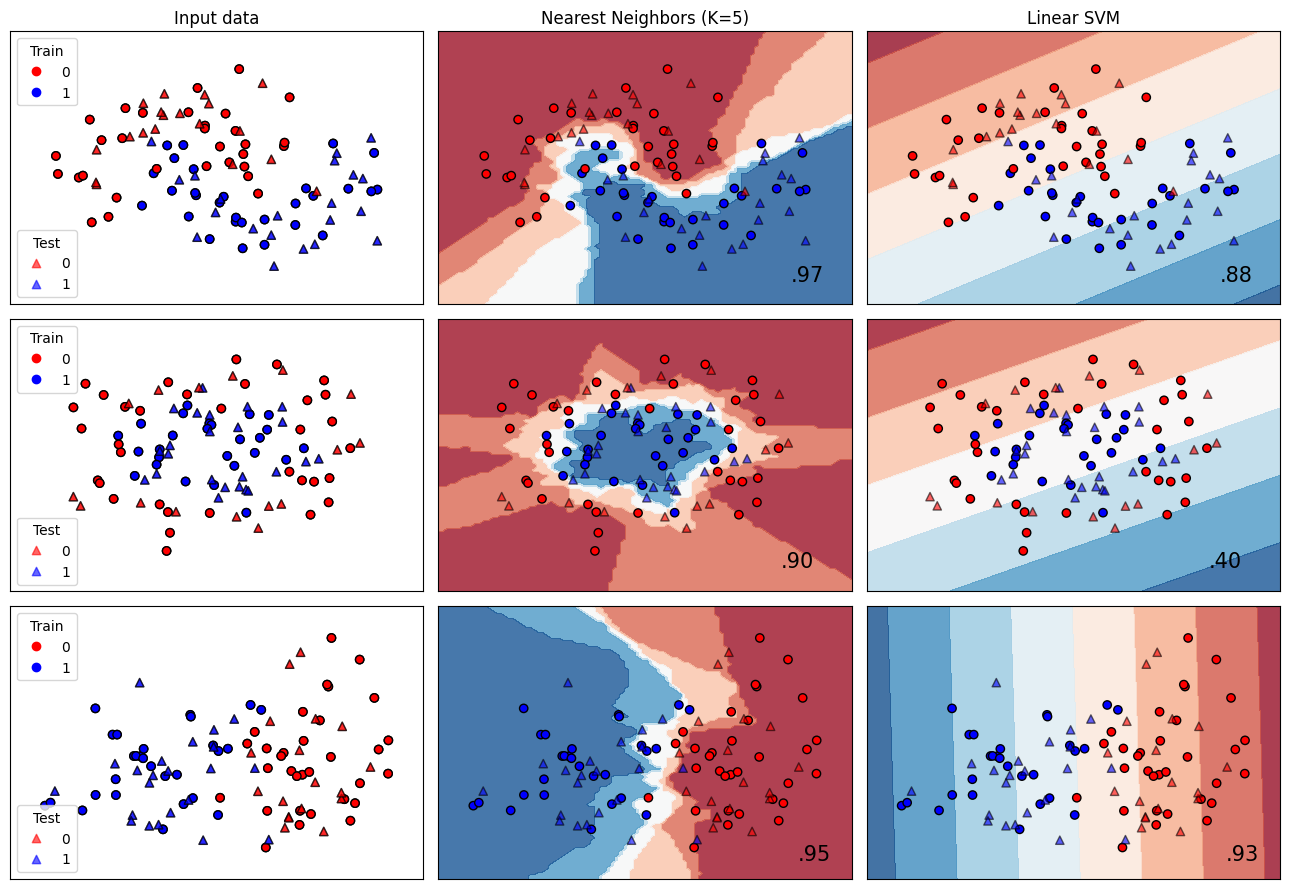
\includegraphics[scale = 0.4]{ClassifierComparrison.png}
    \centering
    \caption{Modified example taken from \url{https://scikit-learn.org/stable/auto_examples/classification/plot_classifier_comparison.html}.}
    \label{fig:ClassifierComparrison}
\end{figure}

\subsection{Generative model}

Evaluating generative models remains a challenging task, as it requires assessing how well the generated samples match the real data distribution. While some data modalities have established evaluation standards, such as ImageNet and Inception v3 in the computer vision domain, others like time series lack widely accepted benchmarks.\newline

The traditional sanity check for generative models is human visual inspection. However, this approach is subjective and varies significantly between data modalities. For example, while most people can easily judge the quality of generated images, interpreting generated time series data often requires domain-specific knowledge. This is one of the obstacles in TSG. Despite this, according to \cite{TimeVQVAE} the most common evaluation protocols in the TSG literature is PCA and t-SNE analyses to visually see similarities of distributions, complemented by quantitative metrics where possible.\newline

Following the approach in \cite{TimeVQVAE}, we employ three primary evaluation metrics in this thesis: Inception Score (IS), Fréchet Inception Distance (FID), and Classification Accuracy Score (CAS).\newline

All the mentioned evaluation metrics depend on a pre-trained classification model. Unlike computer vision, where models like Inception v3 are standard, there is no universally adopted classification model for time series data. However, \cite{wang2016time} proposed a fully convolutional network (FCN) as a baseline model for time series classification. Since the original model is not readily available, we utilize an open-source FCN trained on the UCR Archive, as presented in \cite{TimeVQVAE}, for our evaluations.

\subsubsection{Inception Score (IS)}

The Inception Score (IS) was first introduced in \cite{salimans2016improved} as an automatic method for evaluating the quality of synthetic samples. IS measures the clarity and diversity of generated samples by using a pre-trained classifier to predict labels. The intuition behind IS is that high-quality samples should result in low entropy in the conditional label distribution $p(y|x)$, while diverse samples should lead to high entropy in the marginal label distribution $p(y)$. Thus if the KL-divergence between these distributions are high, the samples should be of high quality. The Inception Score is defined as 

\begin{equation}
    \label{IS}
    {\text{IS}}(\theta) = \exp\left( \mathbb{E}(D_{\text{KL}}(p_\theta(y|\mathbf{x}) || p_\theta(y))) \right).
\end{equation}

In the context of time series, we use a fully convolutional network (FCN) trained on the UCR Archive \cite{TimeVQVAE} to obtain an estimate for $p(y|x)$. For a synthetic dataset $X_{\text{gen}} = \{x_{i,\text{gen}}\}_{i=1}^N$, the marginal label distribution is obtained by averaging across all the synthetic data as follows

\[
    p(y) = \frac{1}{N} \sum_{i=1}^N p(y |x_{i,\text{gen}}).
\]

The primary concern with IS is that it does not use any statistics of real world samples to compare with the statistics of the generated samples. Additionally IS has no mechanism for considering the diversity of generated samples within a class, which stresses the importance of reporting additional metrics that indicate whether the model overfits. 

\subsubsection{Fréchet Inception Distance (FID)}
To address some limitations of IS, the Fréchet Inception Distance (FID) was introduced in \cite{heusel2018gans}. Since then FID has been the standard for assessing generative models \cite{borji2021pros}. FID compares the distributions of real and generated samples using the Fréchet distance, providing a measure of how similar the generated samples are to the real data. For any two probability distributions, $f,g$ over $\R^n$, with finite mean and variances, their Fréchet distance is defined as 
\begin{equation}
    \begin{aligned}
        d_F(f,g) &= \left(\inf_{\gamma \in \Gamma(f,g)} \int_{\R^n\times\R^n}||x-y||_2^2d\gamma(x,y) \right)^{\frac{1}{2}}\\\\
            &= \left(\inf_{\gamma \in \Gamma(f,g)} \E_{(x,y)\sim \gamma} ||x-y||_2^2\right)^{\frac{1}{2}},
    \end{aligned}
\end{equation}
where $\Gamma(f,g)$ is the set of all \textit{couplings} of $f$ and $g$. For two Gaussian distributions, as proven in  \cite{DOWSON1982450}, the Fréchet distance is explicitly computable as
\begin{equation}
    \label{eq:FID Gaussian}
    d(\N(\mu,\Sigma),\N(\mu',\Sigma'))^2 = ||\mu-\mu'||_2^2 + \Tr \left( \Sigma + \Sigma' - 2(\Sigma\Sigma')^{\frac12}\right).
\end{equation}

In FID, the mean and covariance of the feature representations of real and generated samples are computed using a pre-trained model. They argue in \cite{heusel2018gans} that since the Gaussian distribution is the maximum entropy distribution over $\R^n$, for a given mean and covariance, it is a reasonable distribution to assume for the representations. But, despite its usefulness, FID has limitations, such as the Gaussian assumption not always holding true and the need for a large number of samples to estimate the covariance matrix reliably \cite{jayasumana2024rethinking}, \cite{chong2020effectively}.

\subsubsection{Classification Accuracy Score (CAS)}
% \cite{smith2020conditional} report the CAS.
Classification Accuracy Score (CAS) evaluates the model's ability to learn class-conditional distributions. This is done by training a classifier on synthetic data and testing it on real data (Train on Synthetic, Test on Real - TSTR). The process involves generating synthetic samples conditioned on class labels, training a classifier on these samples, and evaluating its accuracy on a real test dataset. High CAS values indicate that the generative model produces samples that capture relevant class-specific features.\newline

In this thesis, we use the Supervised FCN introduced in \cite{TimeVQVAE} to evaluate CAS across all models considered, comparing the results against a baseline model to assess relative performance.

\end{document}